\documentclass[12pt,a4paper]{article}

\usepackage[english]{babel}
\selectlanguage{english}
\usepackage[applemac]{inputenc}
\usepackage{graphicx}
\usepackage{xcolor}
\usepackage{fancyhdr}
\usepackage{latexsym}
\usepackage{amsfonts}
\usepackage{amssymb}
\usepackage{amsmath}
\usepackage{cite}
\usepackage{verbatim}
\usepackage{url}
\usepackage[pdftex]{hyperref}
\hypersetup{
pdfauthor={Alessandra Bonetto, Filippo Sironi, Matteo Villa},
pdfsubject={Formal Methods for Concurrent and Real-Time Systems},
pdftitle={Computer Controller Automatic Transmission},
pdfborder={0 0 0},
colorlinks,
citecolor=black,
filecolor=black,
linkcolor=black,
urlcolor=black
}
\usepackage{sans}
\usepackage{indent�rst}
\usepackage{listings}
%%
%% TRIO+ definition
%%
\lstdefinelanguage{TRIO}{
morekeywords=[0]{class,signature,visible,temporal,domain,domains,items,axioms,vars,formulae,end,import,modules,connections},
keywordstyle=[0]\color{violet}\bfseries,
morekeywords=[1]{state,event,const,TD,total,TI,direct},
keywordstyle=[1]\color{violet},
morekeywords=[2]{Dist,Past,Futr,Lasted,Lasts,WithinP,WithinF,Som,SomP,SomF,Alw,AlwP,AlwF,UpToNow,NowOn},
keywordstyle=[2]\color{blue},
morekeywords=[3]{integer,real},
keywordstyle=[3]\color{green},
morekeywords=[4]{all,ex,and,or,not,implies,iff},
keywordstyle=[4]\color{blue}\bfseries,
morecomment=[s][\color{green}]{/*}{*/},
morecomment=[l][\color{green}]//,
sensitive
}

\begin{document}

\thispagestyle{empty}
\begin{center}
{\huge Politecnico di Milano}
\end{center}
\begin{center}
{\huge Formal Methods for Concurrent and Real-Time Systems}
\end{center}
\vskip 9cm
\begin{center}
{\Large Computer Controller Automatic Transmission}
\end{center}
\vskip 2cm
\begin{center}
{\large Alessandra Bonetto\\Filippo Sironi\\Matteo Villa}
\end{center}
\vskip 2cm
\begin{center}
{\large 2009}
\end{center}

\newpage
\pagestyle{fancy}
\fancyhf{}
\fancyhead[R]{\bfseries\thepage}
\fancyhead[L]{\bfseries\rightmark}
\fancyhead[L]{\bfseries\leftmark}

\newpage
\tableofcontents

\newpage
\listoffigures

\newpage
\lstlistoflistings

\newpage
\section{Big Picture}
\label{Section:Structure}
Figure~\ref{Figure:CCAT} shows the \emph{big picture} of the \emph{Computer Controlled Automatic Transmission} we designed.

\thispagestyle{empty}
\begin{figure}[!p]
\vspace{-3 cm}
\centerline{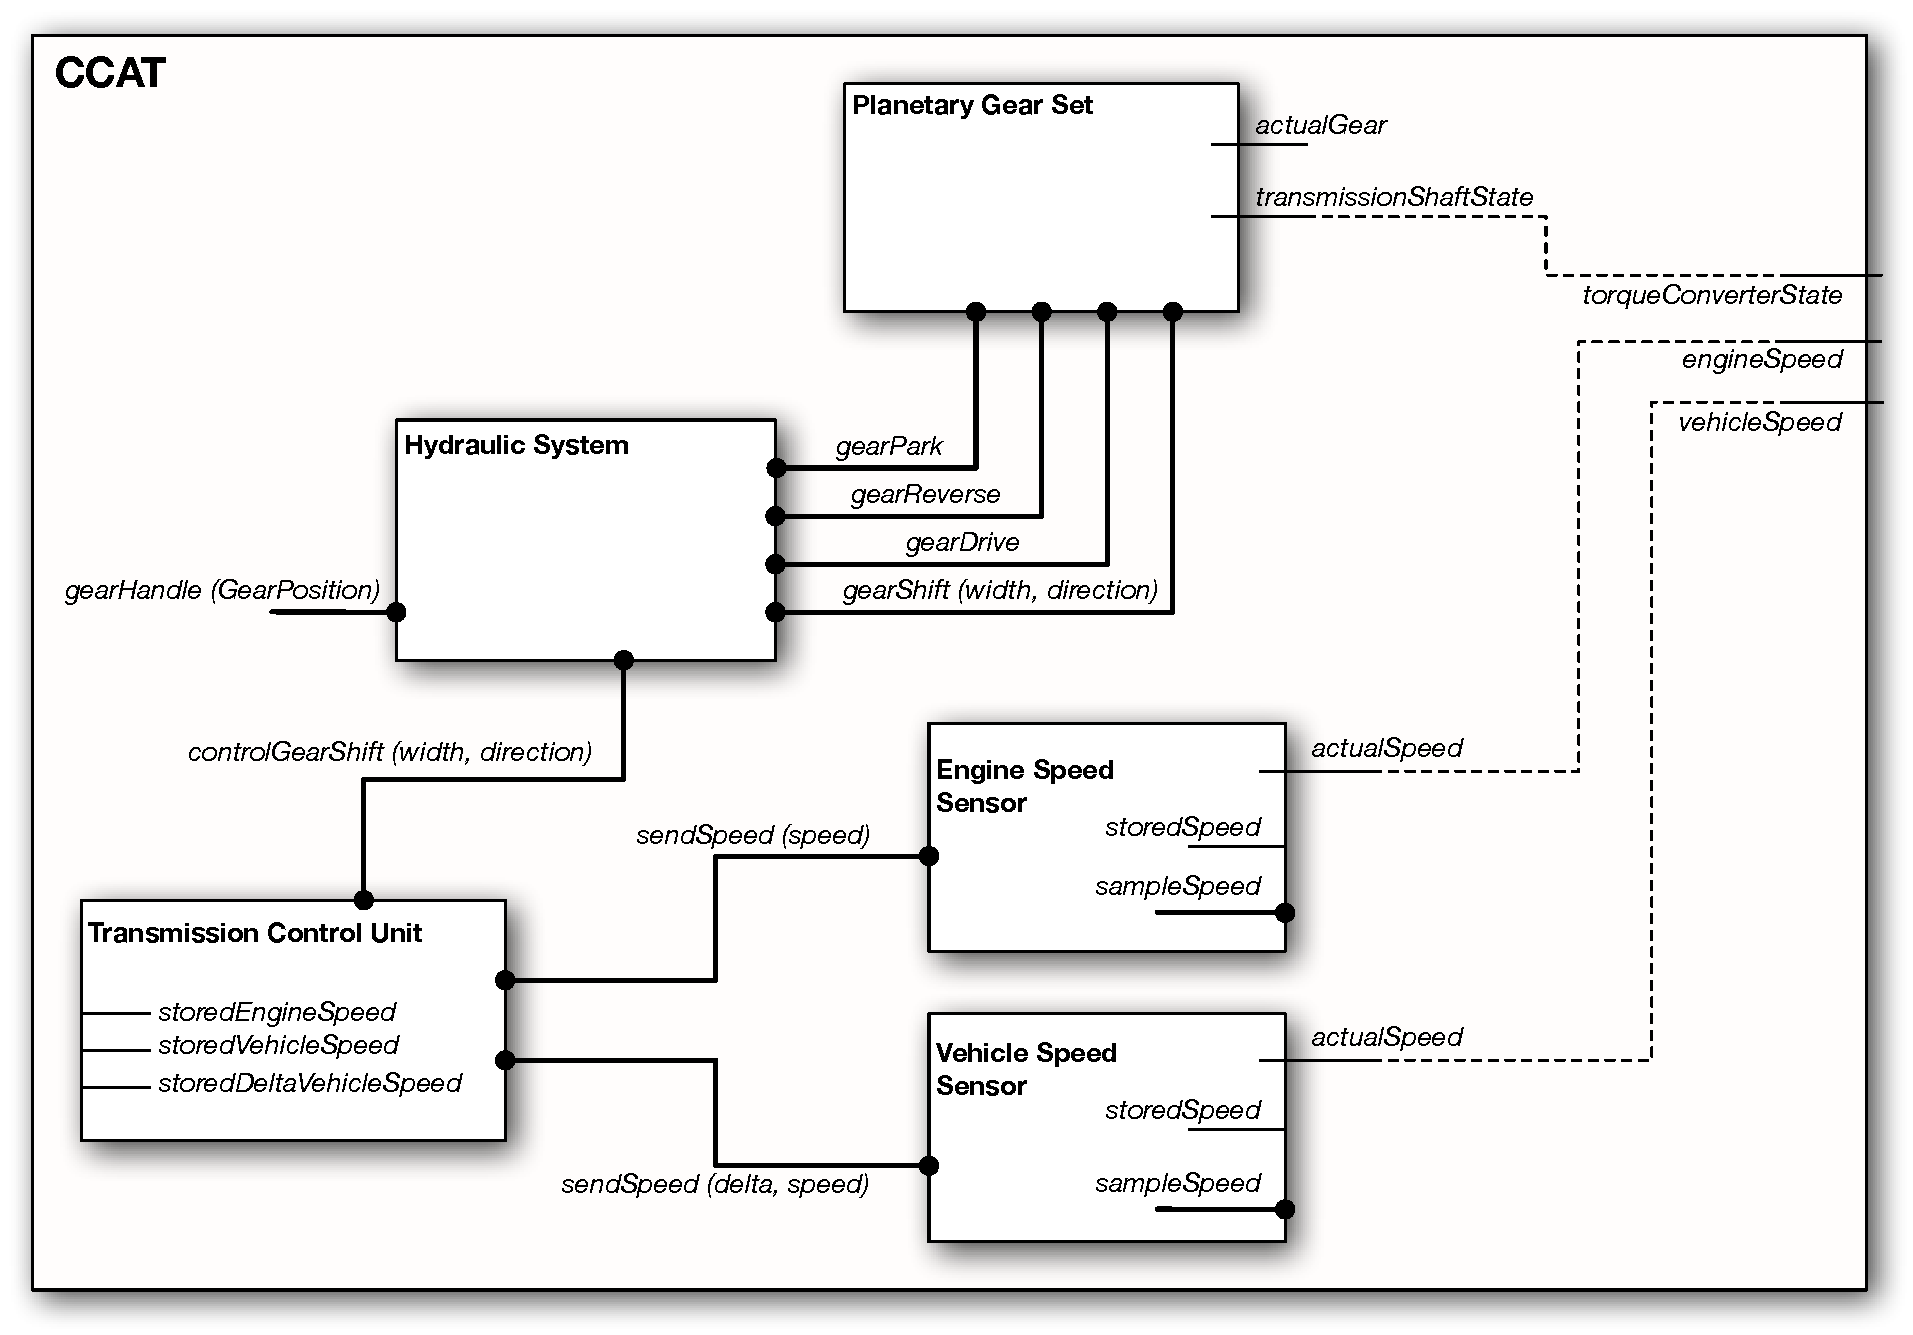
\includegraphics[scale=0.8,angle=-90]{images/CCAT.pdf}}
\caption{Computer Controller Automatic Transmission}
\label{Figure:CCAT}
\end{figure}

\newpage
\section{Vehicle/EngineSpeedSensor Classes}
\label{Section:SpeedSensors}
The \emph{VehicleSpeedSensor} is formalized thanks to the code reported in Listing~\ref{Code:VehicleSpeedSensor} while the \emph{EngineSpeedSensor} is formalized thanks to the code reported in Listing~\ref{Code:EngineSpeedSensor}.

During the formalization of sensors we decided to simplify the design assuming that every time a \texttt{sampleSpeed} event occurs the state variable \texttt{actualSpeed} - which is \texttt{time dependent} and \texttt{total} - is automatically updated with the actual measured speed. This means we don't provide any axioms formalizing this behavior.

Moreover, we specified the starting point of the constant frequency sample chain saying that sometimes in the past there was a \texttt{sampleSpeed} occurrence. Further more, we guarante that \texttt{sampleSpeed} events will accure at constant frequency. In addition, if the sensor has memory we imposed that the \texttt{storedValue} is equal to 0. These can be consider just like the ``initial conditions'' of the system.

At the end, we guaranteed a sensor performs the needed action if and only if a sample event occur.

We didn't write any axioms specifying the fact that a \texttt{sendSpeed} event is mutually exclusive with itself due to the \texttt{total time dependent} parameter it accepts.

\lstinputlisting[language=TRIO,tabsize=4,numbers=left,numberstyle=\small,basicstyle=\small,breaklines,breakatwhitespace,frame=single,caption=VehicleSpeedSensor.trio,label=Code:VehicleSpeedSensor]{../src/VehicleSpeedSensor.trio}

\lstinputlisting[language=TRIO,tabsize=4,numbers=left,numberstyle=\small,basicstyle=\small,breaklines,breakatwhitespace,frame=single,caption=EngineSpeedSensor.trio,label=Code:EngineSpeedSensor]{../src/EngineSpeedSensor.trio}

\newpage
\section{PlanetaryGearSet Class}
\label{Section:PlanetaryGearSet}
The \emph{PlanetaryGearSet} class is formalized thanks to the code reported in Listing~\ref{Code:PlanetaryGearSet}.

The Planetary Gear Set guarantees that every time a gear shift event occurs the \texttt{actualGear} will be maintained until the shift is finished.

Inside this component are defined all axioms limiting gear shifts to effective ones only (e.g. it is impossibile to shift down a gear if \texttt{actualGear} is \texttt{First}.

Moreover, through the formalization of the Planetary Gear Set we impose that we can't receive a gear shift event if we are in the middle of a gear shift. Different gear shifting times are defined for different gears and different steps.

The gears \texttt{Drive}, \texttt{Park}, and \texttt{Reverse} can be selected if and only if the transmission shaft is decoupled from the engine.

The state of the Planetary Gear Set changes if and only if an event occurs.

\lstinputlisting[language=TRIO,tabsize=4,numbers=left,numberstyle=\small,basicstyle=\small,breaklines,breakatwhitespace,frame=single,caption=PlanetaryGearSet.trio,label=Code:PlanetaryGearSet]{../src/PlanetaryGearSet.trio}

\newpage
\section{HydraulicSystem Class}
\label{Section:HydraulicSystem}

\newpage
\section{TransmissionControlUnit Class}
\label{Section:TransmissionControlUnit}

%\bibliographystyle{settings/IEEEtran}
\bibliographystyle{unsrt}
\bibliography{bibliography.bib}

\end{document}
